\documentclass{beamer}
\usepackage[utf8]{inputenc}
\usepackage[T5]{fontenc}
\usepackage[vietnamese]{babel}
\usepackage{graphicx}
\usepackage{amsmath}

% Chọn giao diện (theme) cho slide
\usetheme{Madrid}
\usecolortheme{default}

% ================= TRANG BÌA =================
\title[Cài đặt Perceptron \& MLP]{CÀI ĐẶT PERCEPTRON VÀ MẠNG NƠ-RON NHIỀU LỚP (MLP) TỪ ĐẦU BẰNG NUMPY}
\author[Thiện, Vũ]{
  Đại học Phenikaa \\
  Trường Công nghệ Thông tin Phenikaa \\
  \vspace{0.5cm}
  \textit{Giảng viên hướng dẫn: ThS. Phan Thị Hoài} \\
  \vspace{0.2cm}
  \textbf{Sinh viên thực hiện:} \\
  Ngô Quang Thiện - Nguyễn Hưng Vũ
}
\institute[Phenikaa Uni]{}
\date{}

\begin{document}

\begin{frame}
  \titlepage
\end{frame}

\begin{frame}{Nội dung trình bày}
  \tableofcontents
\end{frame}

% ================= CƠ SỞ LÝ THUYẾT =================
\section{Cơ sở lý thuyết}

\begin{frame}{2.1 Quy ước ký hiệu}
  \begin{itemize}
    \item $X$: Ma trận dữ liệu đầu vào. $x$: Vector đặc trưng.
    \item $W^{(l)}$: Ma trận trọng số lớp $l$. $w$: Vector trọng số.
    \item $b^{(l)}$: Vector bias lớp $l$.
    \item $z$: Giá trị trước hàm kích hoạt. $Z^{(l)}$: Ma trận giá trị trước kích hoạt.
    \item $a$: Đầu ra sau hàm kích hoạt. $A^{(l)}$: Ma trận đầu ra sau kích hoạt.
    \item $\hat{y}$: Giá trị dự đoán. $y$: Nhãn thực tế.
    \item $\delta^{(l)}$: Sai số lan truyền ngược lớp $l$.
    \item $\eta$: Tốc độ học. $\beta$: Hệ số Momentum. $\lambda$: Hệ số L2.
    \item $\mathcal{L}$: Hàm mất mát.
  \end{itemize}
\end{frame}

\begin{frame}{2.2.1 Kiến trúc Perceptron}
  \begin{itemize}
    \item \textbf{Đầu vào:} $\mathbf{x} = [x_1, x_2, \dots, x_n]^T$
    \item \textbf{Trọng số:} $\mathbf{w} = [w_1, w_2, \dots, w_n]^T$
    \item \textbf{Tổng có trọng số:}
    \begin{equation*}
        z = \sum_{i=1}^n w_i x_i + b \quad \text{hay} \quad z = \mathbf{w}^T \mathbf{x} + b
    \end{equation*}
    \item \textbf{Hàm kích hoạt (Step Function):}
    \begin{equation*}
        \hat{y} = f(z) = \begin{cases} 1, & z \ge 0 \\ 0, & z < 0 \end{cases}
    \end{equation*}
    \item \textbf{Cập nhật trọng số:}
    \begin{equation*}
        w_i = w_i + \eta(y - \hat{y})x_i, \quad b = b + \eta(y - \hat{y})
    \end{equation*}
  \end{itemize}
\end{frame}

\begin{frame}{2.2.2 Giới hạn phân tách tuyến tính (Bài toán XOR)}
  \begin{itemize}
    \item Perceptron chỉ phân tách được các dữ liệu tuyến tính (có thể chia bằng 1 đường thẳng/mặt phẳng).
    \item \textbf{Bài toán XOR (Exclusive OR):}
    \begin{table}[H]
    \centering
    \begin{tabular}{|c|c|c|}
    \hline
    $x_1$ & $x_2$ & Output \\
    \hline
    0 & 0 & 0 \\
    0 & 1 & 1 \\
    1 & 0 & 1 \\
    1 & 1 & 0 \\
    \hline
    \end{tabular}
    \end{table}
    \item Dữ liệu XOR phân bố chéo nhau, không thể dùng một đường thẳng phân tách. Do đó Perceptron một lớp không thể giải bài toán này.
  \end{itemize}
\end{frame}

\begin{frame}{2.2.3 Mạng nơ-ron nhiều lớp (MLP) \& Cách giải quyết XOR}
  \begin{itemize}
    \item \textbf{Mạng nơ-ron nhiều lớp (MLP):} Khắc phục hạn chế của Perceptron bằng cách thêm một hoặc nhiều \textbf{lớp ẩn (Hidden Layers)} giữa lớp Input và Output.
    \item Kết hợp với các \textbf{hàm kích hoạt phi tuyến} (như ReLU, Sigmoid), MLP có thể tạo ra các biến đổi không gian phức tạp.
    \item \textbf{Cách MLP giải quyết XOR:}
    \begin{itemize}
        \item Các nơ-ron trong lớp ẩn học cách tạo ra nhiều ranh giới phân tách cục bộ.
        \item Khi kết hợp lại ở lớp Output, chúng tạo thành một \textbf{ranh giới quyết định phi tuyến}, cho phép phân tách hoàn toàn các mẫu XOR mà Perceptron đơn lớp thất bại.
    \end{itemize}
  \end{itemize}
\end{frame}

\begin{frame}{2.3.1 Hàm Sigmoid}
  \begin{itemize}
    \item Biến đổi giá trị đầu vào về khoảng $(0,1)$. Thường dùng cho bài toán phân loại nhị phân.
    \item \textbf{Công thức hàm:}
    \begin{equation*}
        \sigma(z) = \frac{1}{1 + e^{-z}}
    \end{equation*}
    \item \textbf{Đạo hàm:}
    \begin{equation*}
        \sigma'(z) = \sigma(z)\bigl(1 - \sigma(z)\bigr)
    \end{equation*}
  \end{itemize}
\end{frame}

\begin{frame}{2.3.2 Hàm ReLU}
  \begin{itemize}
    \item \textbf{ReLU (Rectified Linear Unit):} Hàm kích hoạt phổ biến ở các Hidden Layer, giúp giảm thiểu hiện tượng mất gradient và tính toán nhanh.
    \item \textbf{Công thức hàm:}
    \begin{equation*}
        f(z) = \max(0, z)
    \end{equation*}
    \item \textbf{Đạo hàm:}
    \begin{equation*}
        f'(z) = \begin{cases} 1, & z > 0 \\ 0, & z \le 0 \end{cases}
    \end{equation*}
  \end{itemize}
\end{frame}

\begin{frame}{2.3.3 Hàm Softmax}
  \begin{itemize}
    \item Dùng ở Output Layer của bài toán phân loại nhiều lớp. Chuyển vector đầu vào thành phân phối xác suất có tổng bằng 1.
    \item \textbf{Công thức tại nơ-ron $c$:}
    \begin{equation*}
        \hat{y}_c = A^{(L)}_c = \frac{e^{z_c^{(L)}}}{\sum_{j=1}^C e^{z_j^{(L)}}}
    \end{equation*}
    \item \textbf{Dạng ma trận:}
    \begin{equation*}
        A^{(L)} = \mathrm{Softmax}\!\left(Z^{(L)}\right)
    \end{equation*}
  \end{itemize}
\end{frame}

\begin{frame}{2.4 Lan truyền thuận (Forward Propagation)}
  \begin{itemize}
    \item Truyền dữ liệu từ Input Layer $\rightarrow$ Hidden Layer $\rightarrow$ Output Layer.
    \item Ở mỗi lớp $l$, tính tổng có trọng số và áp dụng hàm kích hoạt.
    \item \textbf{Công thức tổng quát cho lớp $l$:}
    \begin{align*}
        Z^{(l)} &= W^{(l)} A^{(l-1)} + b^{(l)} \\
        A^{(l)} &= f\left(Z^{(l)}\right)
    \end{align*}
  \end{itemize}
\end{frame}

\begin{frame}{2.5 Hàm mất mát (Loss Function)}
  \begin{itemize}
    \item Đo lường sai lệch giữa dự đoán và thực tế.
    \item \textbf{Mean Squared Error (Hồi quy):}
    \begin{equation*}
        \mathcal{L} = \frac{1}{N} \sum_{i=1}^N (y_i - \hat{y}_i)^2
    \end{equation*}
    \item \textbf{Binary Cross-Entropy (Phân loại nhị phân):}
    \begin{equation*}
        \mathcal{L} = - \frac{1}{N} \sum_{i=1}^N \left[ y_i \log(\hat{y}_i) + (1 - y_i) \log(1 - \hat{y}_i) \right]
    \end{equation*}
    \item \textbf{Categorical Cross-Entropy (Phân loại nhiều lớp):}
    \begin{equation*}
        \mathcal{L} = - \frac{1}{N} \sum_{i=1}^N \sum_{c=1}^C y_{ic} \log(\hat{y}_{ic})
    \end{equation*}
  \end{itemize}
\end{frame}

\begin{frame}{2.6 Lan truyền ngược (Backpropagation)}
  \begin{itemize}
    \item \textbf{Quy tắc đạo hàm dây chuyền:} $\frac{\partial \mathcal{L}}{\partial w} = \frac{\partial \mathcal{L}}{\partial a} \cdot \frac{\partial a}{\partial z} \cdot \frac{\partial z}{\partial w}$
    \item \textbf{Đạo hàm lớp cuối:} $\delta^{(L)} = A^{(L)} - Y$
    \item \textbf{Lan truyền sai số về lớp $l$:}
    \begin{equation*}
        \delta^{(l)} = (W^{(l+1)})^T \delta^{(l+1)} \odot f'(Z^{(l)})
    \end{equation*}
    \item \textbf{Tính Gradient (trên $N$ mẫu):}
    \begin{equation*}
        \frac{\partial \mathcal{L}}{\partial W^{(l)}} = \frac{1}{N} \delta^{(l)} (A^{(l-1)})^T, \quad \frac{\partial \mathcal{L}}{\partial b^{(l)}} = \frac{1}{N} \sum_{i=1}^N \delta_i^{(l)}
    \end{equation*}
  \end{itemize}
\end{frame}

\begin{frame}{2.7 Các thuật toán tối ưu (Optimization Algorithms)}
  \begin{itemize}
    \item \textbf{Stochastic Gradient Descent (SGD):}
    \begin{equation*}
        W^{(l)} = W^{(l)} - \eta \frac{\partial \mathcal{L}_i}{\partial W^{(l)}}, \quad b^{(l)} = b^{(l)} - \eta \frac{\partial \mathcal{L}_i}{\partial b^{(l)}}
    \end{equation*}
    \item \textbf{SGD with Momentum:} Tích lũy gradient các bước trước.
    \begin{align*}
        v_t^{W^{(l)}} &= \beta v_{t-1}^{W^{(l)}} - \eta \frac{\partial \mathcal{L}}{\partial W^{(l)}} \\
        W_t^{(l)} &= W_{t-1}^{(l)} + v_t^{W^{(l)}}
    \end{align*}
  \end{itemize}
\end{frame}

\begin{frame}{2.8 Regularization L2}
  \begin{itemize}
    \item Thêm phần phạt vào hàm mất mát để chống Overfitting (Weight Decay).
    \item \textbf{Hàm mất mát mới:}
    \begin{equation*}
        \mathcal{L}' = \mathcal{L} + \frac{\lambda}{2N} \sum_{l=1}^L ||W^{(l)}||_F^2
    \end{equation*}
    \item \textbf{Cập nhật trọng số:}
    \begin{equation*}
        W^{(l)} = W^{(l)} - \eta \left( \frac{\partial \mathcal{L}}{\partial W^{(l)}} + \frac{\lambda}{N} W^{(l)} \right)
    \end{equation*}
  \end{itemize}
\end{frame}

% ================= KẾT QUẢ THỰC NGHIỆM =================
\section{Kết quả thực nghiệm}

\begin{frame}{3.1 Cài đặt Perceptron đơn giản và bài toán XOR}
  \begin{columns}
    \begin{column}{0.5\textwidth}
      \begin{itemize}
        \item Huấn luyện Perceptron 1 lớp với Step Function.
        \item Mô hình \textbf{không hội tụ}, Loss không giảm về 0, độ chính xác 75\%.
        \item Perceptron chỉ vẽ được 1 đường thẳng tuyến tính, không tách được $(1,1)$.
      \end{itemize}
    \end{column}
    \begin{column}{0.5\textwidth}
      \begin{figure}
        \centering
        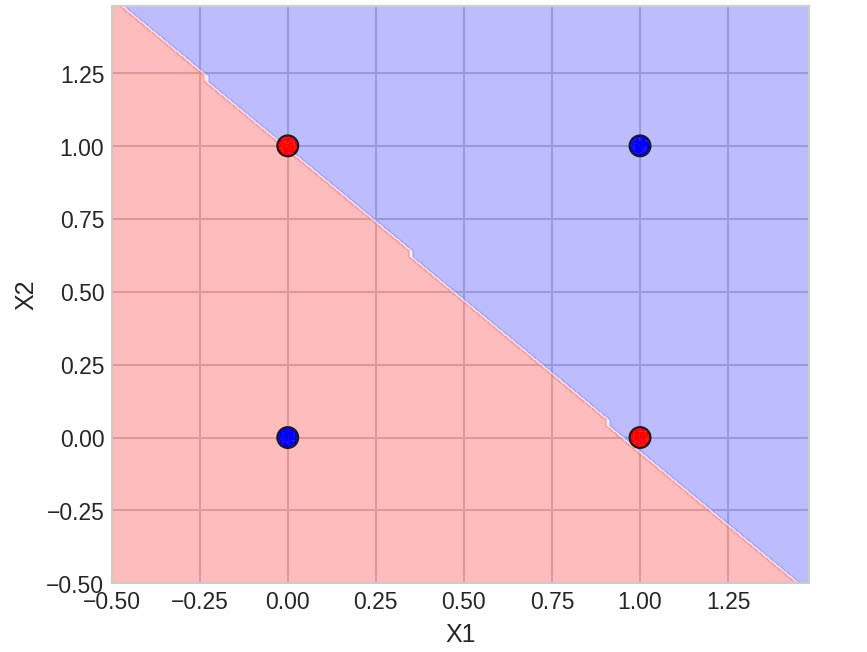
\includegraphics[width=\textwidth]{bao_cao_latex/40.jpg}
        \caption{Perceptron trên XOR}
      \end{figure}
    \end{column}
  \end{columns}
\end{frame}

\begin{frame}{3.2 Đánh giá kết quả cài đặt thuật toán MLP}
  \begin{columns}
    \begin{column}{0.5\textwidth}
      \begin{itemize}
        \item Cài đặt MLP bằng NumPy. Hỗ trợ tùy chỉnh số lớp, số nơ-ron.
        \item Hỗ trợ Forward Propagation, Backpropagation bằng ma trận.
        \item Các hàm kích hoạt: Sigmoid, ReLU, Softmax hoạt động đúng như thiết kế toán học.
      \end{itemize}
    \end{column}
    \begin{column}{0.5\textwidth}
      \begin{figure}
        \centering
        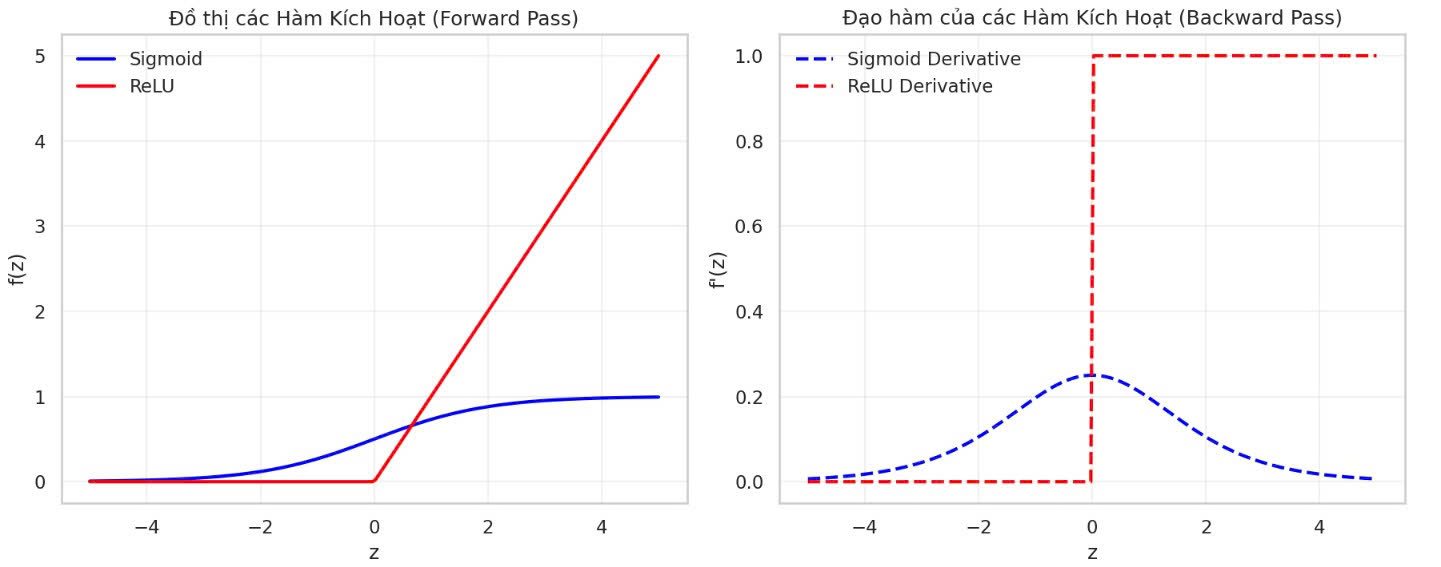
\includegraphics[width=\textwidth]{bao_cao_latex/41.jpg}
        \caption{Các hàm kích hoạt \& đạo hàm}
      \end{figure}
    \end{column}
  \end{columns}
\end{frame}

\begin{frame}{3.3 Đánh giá trên bài toán XOR}
  \begin{columns}
    \begin{column}{0.4\textwidth}
      \begin{itemize}
        \item \textbf{Kiến trúc:} 2 Input - 4 Hidden - 1 Output.
        \item \textbf{Kết quả:} Phân loại đúng 100\%. MLP khắc phục được giới hạn tuyến tính, tạo ra ranh giới phi tuyến.
        \item Hàm ReLU hội tụ nhanh hơn Sigmoid.
      \end{itemize}
    \end{column}
    \begin{column}{0.6\textwidth}
      \begin{figure}
        \centering
        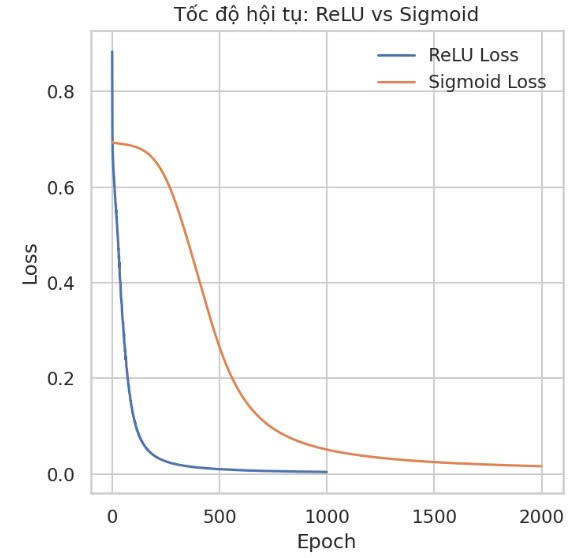
\includegraphics[width=0.7\textwidth]{bao_cao_latex/42.jpg}
        \vspace{0.2cm}
        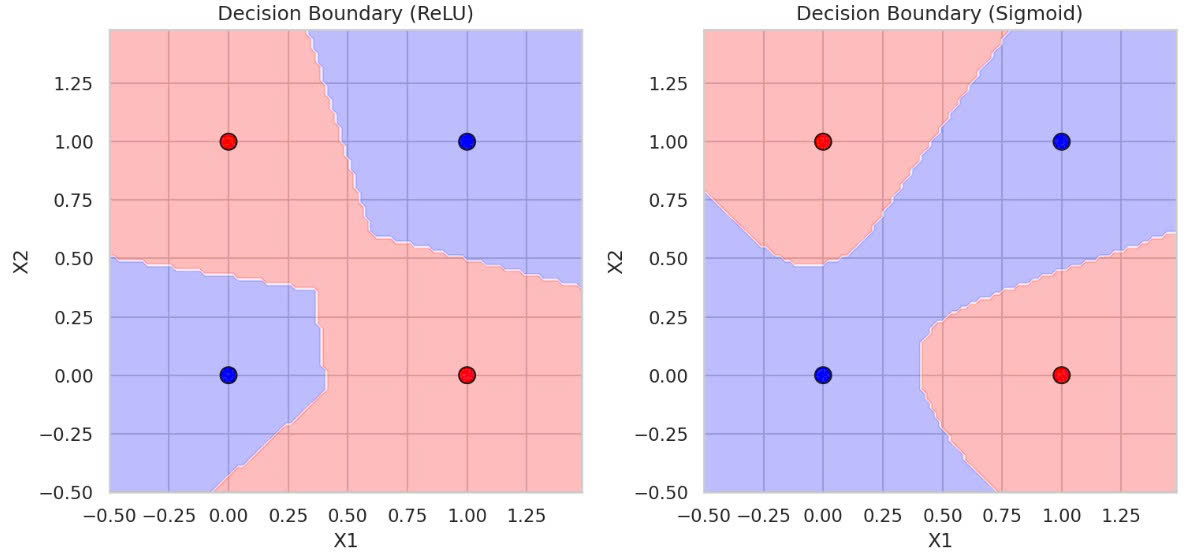
\includegraphics[width=0.7\textwidth]{bao_cao_latex/43.jpg}
        \caption{Ranh giới \& Loss trên XOR}
      \end{figure}
    \end{column}
  \end{columns}
\end{frame}

\begin{frame}{3.4 Đánh giá trên tập dữ liệu Iris}
  \begin{columns}
    \begin{column}{0.45\textwidth}
      \begin{itemize}
        \item \textbf{Kiến trúc:} 4 Input - 8 Hidden (ReLU) - 3 Output (Softmax).
        \item Dữ liệu chuẩn hóa, One-hot nhãn, chia Train(80\%)/Test(20\%).
        \item \textbf{Kết quả:} Hội tụ sau 600 epochs. Độ chính xác đạt 96\% - 100\%.
      \end{itemize}
    \end{column}
    \begin{column}{0.55\textwidth}
      \begin{figure}
        \centering
        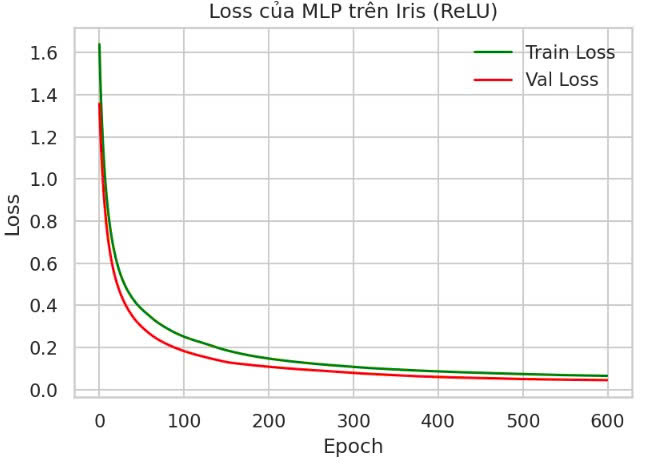
\includegraphics[width=\textwidth]{bao_cao_latex/44.jpg}
        \caption{Huấn luyện MLP trên Iris}
      \end{figure}
    \end{column}
  \end{columns}
\end{frame}

% ================= THỰC NGHIỆM MỞ RỘNG =================
\section{Thực nghiệm mở rộng}

\begin{frame}{4.1 Đánh giá hiệu quả của thuật toán tối ưu SGD với Momentum}
  \begin{columns}
    \begin{column}{0.4\textwidth}
      \begin{itemize}
        \item So sánh SGD và SGD with Momentum ($\beta=0.9$).
        \item \textbf{Kết quả:} Momentum giảm Loss nhanh hơn rất nhiều, đạt khoảng 0.05 sau 100 epochs, trong khi SGD mất 300 epochs chỉ để về 0.18.
      \end{itemize}
    \end{column}
    \begin{column}{0.6\textwidth}
      \begin{figure}
        \centering
        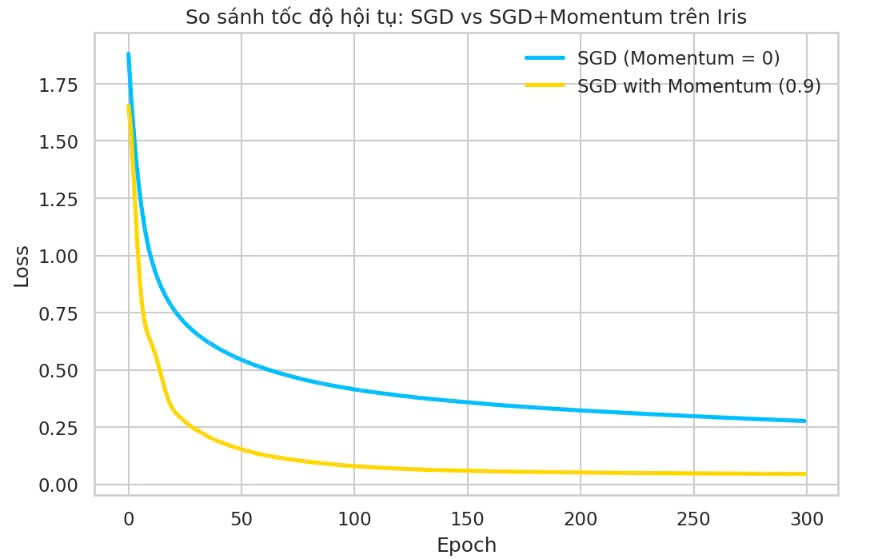
\includegraphics[width=\textwidth]{bao_cao_latex/45.jpg}
        \caption{SGD vs SGD+Momentum}
      \end{figure}
    \end{column}
  \end{columns}
\end{frame}

\begin{frame}{4.2 Ảnh hưởng của số lượng lớp ẩn (Hidden Layers)}
  \begin{columns}
    \begin{column}{0.5\textwidth}
      \begin{itemize}
        \item \textbf{1 lớp:} Hội tụ chậm.
        \item \textbf{2 lớp (4-32-16-3):} Nhanh \& tối ưu nhất.
        \item \textbf{3 lớp:} Cải thiện cực ít nhưng tốn tài nguyên.
      \end{itemize}
    \end{column}
    \begin{column}{0.5\textwidth}
      \begin{figure}
        \centering
        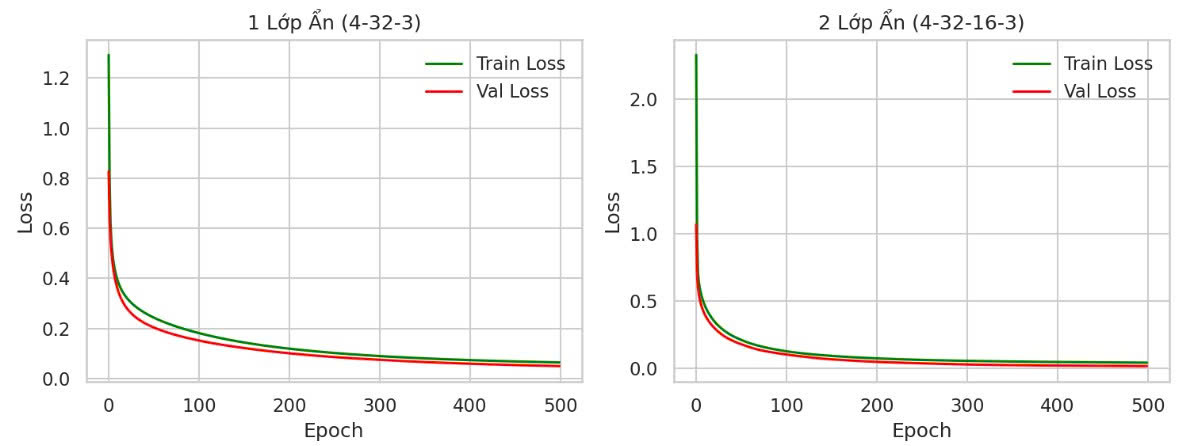
\includegraphics[width=0.8\textwidth]{bao_cao_latex/46.jpg}
        \vspace{0.1cm}
        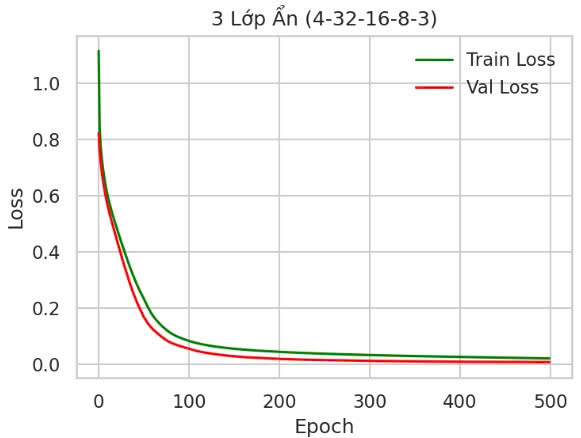
\includegraphics[width=0.8\textwidth]{bao_cao_latex/47.jpg}
      \end{figure}
    \end{column}
  \end{columns}
\end{frame}

\begin{frame}{4.3 Đánh giá hiệu quả của L2 Regularization}
  \begin{columns}
    \begin{column}{0.45\textwidth}
      \begin{itemize}
        \item Dùng mạng lớn (4-64-32-3) trên dữ liệu ít (30 mẫu) để ép Overfitting.
        \item \textbf{Không L2:} Train Loss $\rightarrow$ 0, Val Loss cao (Overfitting).
        \item \textbf{Có L2 ($\lambda=0.15$):} Val Loss giảm tiếp, thu hẹp khoảng cách. L2 chống Overfitting tốt.
      \end{itemize}
    \end{column}
    \begin{column}{0.55\textwidth}
      \begin{figure}
        \centering
        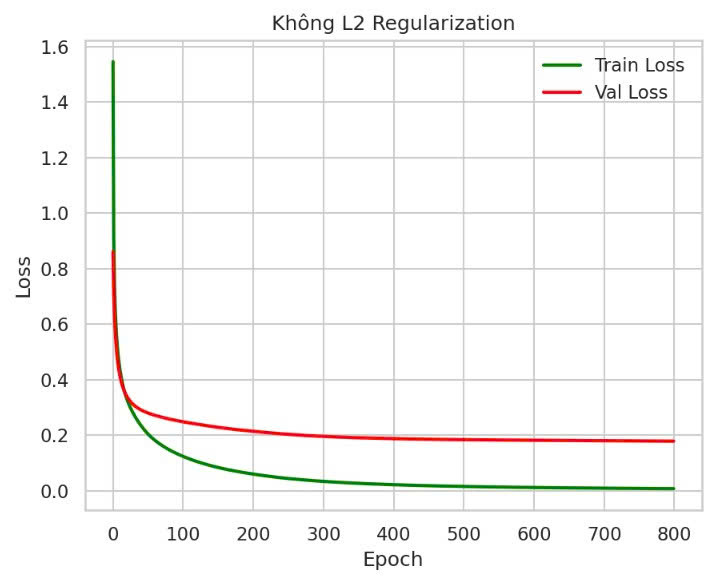
\includegraphics[width=0.8\textwidth]{bao_cao_latex/49.jpg}
        \vspace{0.1cm}
        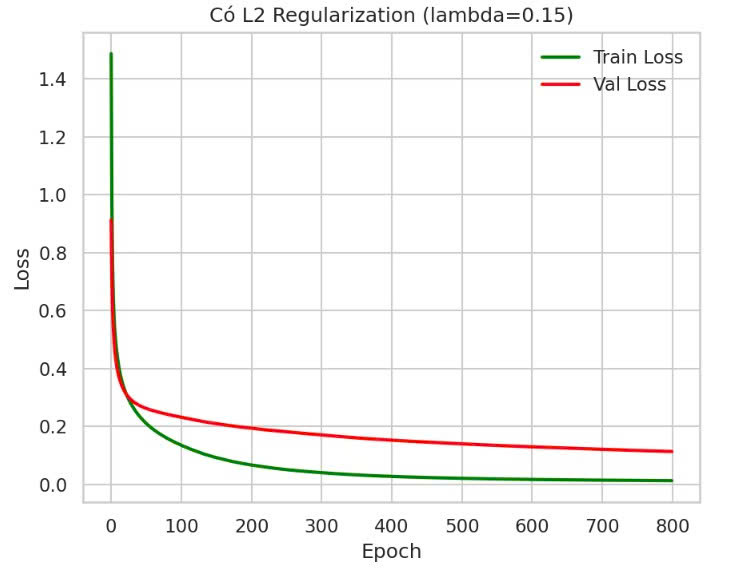
\includegraphics[width=0.8\textwidth]{bao_cao_latex/50.jpg}
      \end{figure}
    \end{column}
  \end{columns}
\end{frame}

\end{document}
